\chapter{Results}\label{results}

\section{Fine-tuning Task}
The fine-tuning task of the BanglaBERT model is very critical for our research as it was determined to be the ground truth for our Natural Langauge Processing-based approach to sentiment analysis. Our model yields a better performance on the training dataset. During the training, we used cross-validation to validate the model against a completely unknown dataset so that the model can learn better. The performance achieved by our model is described in the tables below:

\begin{table}[H]
    \begin{center}
        \begin{tabular}{|l|l|}
        \hline
            \textbf{Metrics}     &   \textbf{Value}  \\ \hline
            Evaluation Accuracy  &   0.744           \\  \hline    
            Evaluation F1 Score  &   0.699           \\  \hline    
            Evaluation Precision &   0.713           \\  \hline    
            Evaluation Recall    &   0.698           \\  \hline    
            Evaluation Loss      &   0.64           \\  \hline    
        \end{tabular}
        \caption{Evaluation Performance Results for BanglaBERT}
        \label{table_banglabert_eval}
    \end{center}
\end{table}

\begin{table}[H]
    \begin{center}
        \begin{tabular}{|l|l|}
        \hline
            \textbf{Metrics}     &   \textbf{Value}  \\ \hline
            Prediction Accuracy  &   0.8376           \\  \hline    
            Prediction F1 Score  &   0.8375           \\  \hline    
            Prediction Precision &   0.8377           \\  \hline    
            Prediction Recall    &   0.8375           \\  \hline
            Train Loss           &   0.7038           \\  \hline    
        \end{tabular}
        \caption{Test Performance Results for BanglaBERT}
        \label{table_banglabert_test}
    \end{center}
\end{table}



\section{Natural Language Processing Approach}
The bar graph and the histogram below denote the total number of positive and negative comments received from the viewers. Figure \ref{fig_comment_type} shows the total number of comments from each class collected from our dataset. It is quite evident that the positive comments are way more in number than the negative ones. The histogram shown in figure \ref{fig_comment_hist} denotes the distribution of the comments in terms of the polarity value.

\begin{figure}[H]
    \begin{center}
        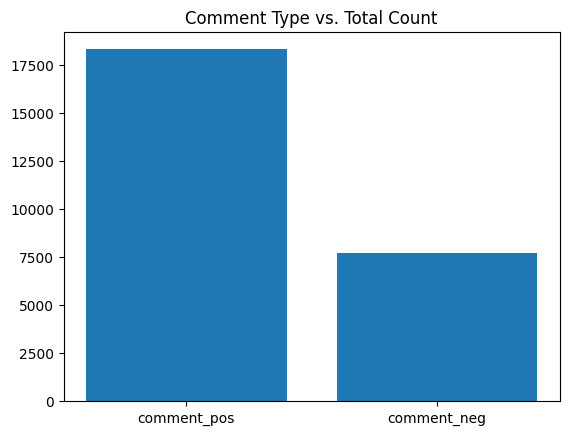
\includegraphics[width=0.6 \linewidth]{figures/comment_type.png}
        \caption{Distribution of positive and negative comments}
        \label{fig_comment_type}
    \end{center}
\end{figure}

\begin{figure}[H]
    \begin{center}
        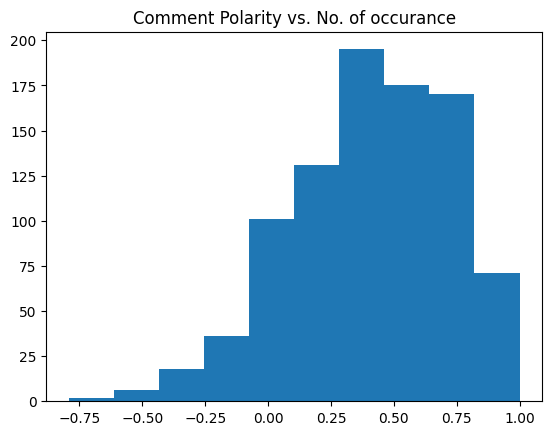
\includegraphics[width=0.6 \linewidth]{figures/comment_polarity.png}
        \caption{Distribution of comments in terms of polarity}
        \label{fig_comment_hist}
    \end{center}
\end{figure}

\section{Interaction Based Approach}
The interaction-based approach proposed in this thesis provides high-level insights into the overall food review situation in social media. The bar graph shown in figure \ref{fig_polarity_class} shows the total number of videos belonging to each of the polarity classes described in chapter \ref{methodology}. The histogram shown in figure \ref{fig_polarity_dist} denotes the polarity distribution of the food review posts.

\begin{figure}[H]
    \begin{center}
        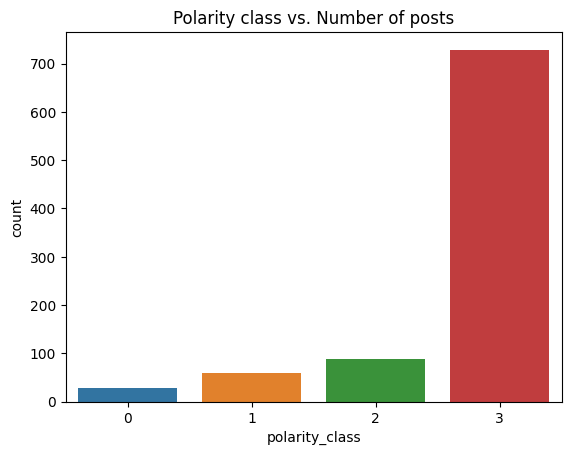
\includegraphics[width=0.65 \linewidth]{figures/polarity_class_vs_count.png}
        \caption{Distribution of posts in terms of polarity class}
        \label{fig_polarity_class}
    \end{center}
\end{figure}

\begin{figure}[H]
    \begin{center}
        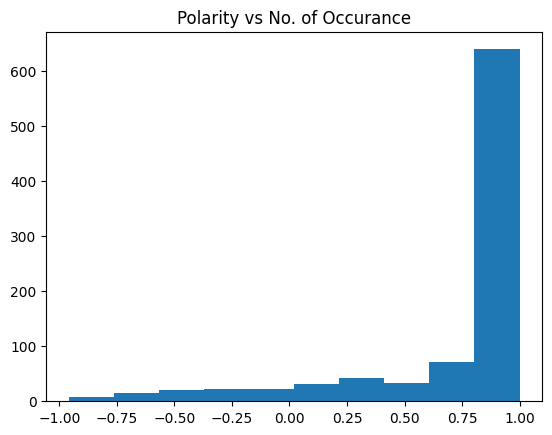
\includegraphics[width=0.65 \linewidth]{figures/polarity_distribution.png}
        \caption{Distribution of posts in terms of polarity score}
        \label{fig_polarity_dist}
    \end{center}
\end{figure}

From both approaches, we find significant insights into the sentiment related to food reviews in the social media domain in Bangladesh. From the interaction-based approach, we can see that more than 90\% of the food review posts contain positive reactions, indicating a positive sentiment. The number of posts decreases along with a lower polarity score, meaning the minimum number of posts shows negative polarity.

On the other hand, the Natural Language Processing-based approach shows a bit different insights. The maximum number of posts contains a polarity score between 0.25 to 0.5. There exist lower high polarity posts than those of medium polarity. And here also, the number of posts decreases along with the polarity level.

Both of the approaches proposed and implemented in this paper indicate a positive sentiment of the food review ecosystem of social media in Bangladesh. Interaction and comments posted by the viewers of the top food vloggers and influencers indicate that there is positive sentiment regarding the overall food review-related content shared in the social media space of Bangladesh.
